\documentclass[a4wide, 10pt]{article}
\usepackage{a4, fullpage}
\usepackage{graphicx}
\usepackage{subcaption}

\setlength{\parskip}{0.3cm}
\setlength{\parindent}{0cm}

\begin{document}

\title{WebApps Final Report 2013 \\
       Quilt}
\author{Briony Goldsack \and Richard Jones \and Anna Thomas \and Eleanor Vincent}
\date{\today}         
\maketitle            

\section{Abstract}

This report will detail the requirements and targets of our web application, Quilt, the design choices involved and its implementation. Furthermore, we shall evaluate our project management and learning experience from this task as well as the future of the application. This report has been written to support the final presentation and demonstration of the application.

\section{Motivation}
% An introduction to the project
Quilt is a social application to improve the sharing and storage of information on the internet. The inspiration came from the idea of 'bookmarks' within a browser and past experiences when sharing information during research projects. Currently, the most used method of sharing websites of interest is to use a medium such as Facebook's Chat application to paste a collection of links. We identified several issues that arose from this practice: links quickly become lost within the chat history or simply forgotten as the conversation progresses; they are purely text with little meaning; and there is no way of highlighting the areas of the website you found particularly useful or interesting in a way that is easy for the other participant to find. This equates to a messy and ultimately inefficient way of sharing information. Quilt's aim is to streamline this process.

% Requirements
By enabling the ability to 'tag' URLs, users are able to remind themselves of why a link held initial interest. Furthermore, users can collect a large selection of websites under one tag, which can then be shared with other users. Image thumbnails, rather than pure text, allow users to obtain an idea of the subject matter before actually clicking on a link, and also allow users to highlight the specific parts of the page that holds interest, for both themselves and friends. This enables them to browse those websites with the most relevance or interest first and less time is wasted gauging a page's overall use. We also wanted a search feature, which would take a tag as an input and return the bookmarks and groups the user has created with that tag. Quilt has been created as an iPad application, but we wanted to include a browser plug-in so users can 'bookmark' a website without leaving the page, so will not interrupt the fluidity of browsing the internet and makes using our application more natural and appealing. To further the marketability of Quilt, we also aimed to create a graphical user interface in line with the many applications and apple products available on the iStore at the moment.

%Target System
Quilt has been created as an iPad application to reflect the current trend of most socialites within society. The idea behind Quilt is the speed and fluidity of sharing things of interest, and the iPad reflects this concept in its ability to be fast and mobile. By nature, whilst some may use their iPad for solid work, many iPad users engage with their iPad as a means for quick internet research and the ease of communicating with their friends through a variety of social media outlets; Quilt fits perfectly within this scope. The iPad is thought to be more stable and easier to use than Android tablets, tending to be be simpler with applications consistent in their appearance and behaviour. Furthermore, by making an application for the Apple market we only needed to support a limited number of devices, therefore making it easier to fix bugs. In addition we favoured the sleek style of iPad and iPhone applications.

% Target Audience
Quilt has been designed to be appealing to a wide range of users, the expected average age to fall around the young to mid twenties, and for a huge variety of technical capabilities. The application has been designed with simplicity in mind for this reason but will include convenient short cuts for those who are very adept with the product.


\section{Project Management}

\subsection{Language Specification}
% Implementation languages
Objective-C is the primary programming language when writing software for OS X and iOS. It is a superset of the C programming language, but has the advantages of providing object-orientated capabilities and a dynamic runtime meaning that an Objective-C application can load an interface, connect objects in the interface to the application code, then run the correct method once the UIButton is pressed without the need to recompile. Objective-C is perfect for use within apps as it is compiled to run at very fast speeds. Furthermore, the framework classes of Cocoa and Cocoa Touch, Apple's GUI libraries, which some of the features of our application rely on, require coding with Objective-C. We felt Objective-C's provision of error objects was particularly important as a good web application should plan for errors and decide how best to handle them to present the best possible user experience when something goes wrong. In addition, we required a way of managing the lifetime of objects for which Objective-C provides an Automatic Reference Counting feature within the compiler.

PHP is probably the most popular scripting language on the web. We chose PHP as it was easy to integrate with our web application to provide ways of interacting with our users, for example, creating a login, maintaining sessions, and implementing messaging systems. PHP also allowed us to utilise the infrastructure already in place on the DOC servers and communicate between the database and our application. 
 
One of the main reasons we chose to use JSON as our data transmission format is because Apple's Objective-C libraries provide built in support for this language. JSON is highly versatile and can be parsed and used by lots of programming languages. An alternative to JSON could have been XML, however JSON is less verbose, so it is quicker to write and we also found it quicker to read. Furthermore, JSON can be parsed trivially using the eval() procedure in JavaScript, and includes arrays. 

The database was coded using SQL. PostgreSQL is the world's most advanced open source database.

\subsection{Design Process}

Our strategy for design revolved around a definition statement created early on in our design process in order to clarify our idea and ultimately create a coherent product that people want to own. Our definition statement is a concise and concrete declaration of our application's main purpose and its intended audience.

Quilt definition statement: An information sharing tool for group research and social interaction.

This definition statement stemmed from our identification of the current problems with information sharing and allowed us to put together our list of requirements (tags, images, friends etc.) as well as our target systems and target audience [see Motivation].

Given that Quilt is predominantly an iPad application there are a couple of different design aspects that were important to consider throughout development in order to produce a quality application.

Battery life is one of the first points to consider on any mobile device. It is important to design a product that does not drain the life of the device too rapidly, or else the user may be less likely to use the product. Quilt has elected to group together temporally local network accesses as having many small network communications would drain the battery life much quicker, due to the constant use of the networking hardware. Grouping the accesses together means more idle time for the networking hardware and so less battery life spent.

A further networking issues which we faced was that we needed to sort the bookmarks by a number of categories - almost every field within the database. That is to say, it is required that we are able to search locally by tag, size, name etc. The issue with this is that is must be done locally and cannot be delegated to the database itself. The reason for this being that the main bottleneck is network performance, which could be incredibly poor. Even given one million bookmarks, stored in 256 bits each, this is still only 32MB of space, so we could could not justify not storing the information locally and simply receiving updates from the server. 256 bits can be considered a conservative estimate but even doubling the space requirement per bookmark, one million bookmarks would still only need 64MB of space - the size of a small video - which is not incredibly significant, thus the decision remains to store information locally and only send updates via the network, thereby simply syncing the database together with the iPad. Furthermore, holding as many bookmarks as possible locally means that network accesses are minimised which increases the responsiveness of the application. To support this is a multitude of data structures, such as a dictionary to map tags with bookmarks and a search trie to check tag existence and to search existing tags.

Once the physical aspects of the device have been considered we move onto the discussion of the virtual aspects of the application. Before the appearance of the application is fully considered the usability of the application must be considered and tested. iOS users are accustomed to the appearance and behaviour of the built-in applications, so they tend to expect similar experiences in the applications they download, and so the design choices behind the GUI are crucial to the appeal of our applications and its usability. Quilt will be making full use of the touch gestures available to the device to ensure it is an intuitive experience for the user; the structure will be clean and easy to navigate, user feedback will be subtle, but clear with precise, fluid animations. It is important to comply with other Apple products as users dislike being forced to learn new procedures that don't transfer to any other applications. Alongside this are such features as persistent logins and bookmark creation methods. In a similar vein to how applications such as Facebook and Twitter allow the user to remain logged in to their account permanently (entering an offline/idle state when the application is closed on the iPad so as not to appear permanently online), Quilt will allow users to use the application without logging in with each and every access. The code in place ensures proper authentication of the user through use of the cookies provided by internet services, so every effort is in place to stop users having their accounts hijacked by those with malicious intent. 


\begin{figure}
        \centering
        \begin{subfigure}[b]{0.4\textwidth}
                \centering
                \includegraphics[width=\textwidth]{"screenshots/WebApps Portrait Mock-Up"}
                \caption{Portrait}
        \end{subfigure}%
        ~ %add desired spacing between images, e. g. ~, \quad, \qquad etc.
          %(or a blank line to force the subfigure onto a new line)
        \begin{subfigure}[b]{0.4\textwidth}
                \centering
                \includegraphics[width=\textwidth]{"screenshots/WebApps Landscape Mock-Up"}
                \caption{Lanscape}
        \end{subfigure}
        \caption{Design Mock-Ups}\label{fig:design}
\end{figure}

To improve the user experience even such small points as username choice feedback as been implemented [see figure 1]. In an initial iteration of the product the user would not be aware if their username was available until after submitting their form. In Quilt's current iteration the text will change colour after their cursor has left the field box to indicate whether the username in question is available or not. This is a subtle point but does a great deal to improve the users sign-up experience. Similarly, on registering, if the user inputs two different passwords, the text will change colour to let them know of the error sooner rather than later.

\begin{figure}
        \centering
        \begin{subfigure}[b]{0.4\textwidth}
                \centering
                \includegraphics[width=\textwidth]{"screenshots/Unavailable User"}
                \caption{Register Username}
        \end{subfigure}%
        ~ %add desired spacing between images, e. g. ~, \quad, \qquad etc.
          %(or a blank line to force the subfigure onto a new line)
        \begin{subfigure}[b]{0.4\textwidth}
                \centering
                \includegraphics[width=\textwidth]{"screenshots/Incorrect Pass"}
                \caption{Register Password}
        \end{subfigure}
        \caption{Register New Account}\label{fig:login}
\end{figure}

Behind this it was important to have a strong, usable database structure to hold all of the necessary information. In the initial iteration of the application the database had only three tables - Users, Bookmarks, and Groups. Users simply contained their username and a password. Bookmarks held a post id, the url, priority sizes, the owner and an array field for the associated tags. Similarly Groups only held a group id and then an array for the members of the group. Initially this seemed adequate but it soon became evident that the use of arrays was difficult to add to simply and there was a situation where the syntax broke down and made the method unusable. To fix this the array was extracted out to become its own table within the database. 

To demonstrate, the Bookmark table was taken and Tags was extracted into its own table. The Tags table simply contains two columns, post id and tag, wherein each row is one tag linked to whichever post is specified. This makes querying tags very simple as you need only return the tags of the table associated with the post id you are asking about and the database will simply return an array of your tags, rather than a single element array containing an array of your tags, which was the case with the initial set-up. The other tables with this relationship are Groups and Group Members, Users and Friends, and Bookmarks and Bookmark Visibility. Users has also been improved to contain both a user id as well as a username for session authentication and holds a hash of the user's password. This is much more secure than simply holding the user's password as, should the database be compromised, the hacker would require the algorithm used to hash the password to be able to access the user's account. A salt column is also present for later, further, improvements to password security; the idea being that a salt is randomly generated for the user, hashed, and connected to their given password before the hash algorithm. This means the hacker would require to know both the algorithm for the hash, and the algorithm to generate the salt before they can backtrack to the original password.

\subsection{Back-up systems}

Git was chosen as our source control and back-up system for several reasons. Git's branching model allows users to have multiple local branches that can be entirely independent of each other and the creation, merging and deletion of these branches is fast. This was ideal for such a group project as Quilt as it enabled us to experiment with different ideas without fear of breaking existing features and losing  previous work. Furthermore, as everything is local when using Git, operations such as 'fetch', 'pull' and 'push' are fast and enabled offline project work, which improved productivity as we were able to work while on trains or planes.  

A crucial feature of Git is that it is distributed. This meant that when we were using a centralised work-flow, every user had a full backup of the main server, each of which could be pushed up to replace the main server in the event of a crash or corruption. There is no single point of failure as there existed multiple clones of the repository on multiple machines. Another major factor for choosing Git was the expansion to GitHub, which provided a friendly user-interface and allowed us to fork from other GitHub user's repositories (i.e. ViewDeck [see acknowledgements]) and streamline the overall management of the project.

\subsection{Group Structure}

Overall the group has worked very effectively with one another. The work has been evenly distributed with everyone having a specific area that they have dealt with over the course of the project. 

So far as specific responsibility is concerned, Richard is considered the main organiser of the group, being the one to control the interactions between front-end and back-end and having the overall knowledge of the direction of the project and which areas have the highest priority at any one time. Eleanor has been the main organiser of the source control, ensuring that logs are correct and useful, aiding other members with git related issues, and keeping the main 'TODO' documentation relevant.

Regarding physical work, the dynamic of the group has been relatively fluid thanks to the strong communication between all of the members. The main split of work has been Anna and Briony working predominantly on UI aspects of the application, understanding objective-C and Xcode. Richard handled networking code and Eleanor dealt with the Database structure and server side code. As mentioned previously, there has been much overlap between these areas. In the early stages of the project, UI elements were less crucial so those with that role were assisting with the networking elements. Later on when server side code had been mostly completed, those with that role moved on to create various graphical mock-ups up the product for use by the UI members and also test the various elements of the application. In the early stages, server side and networking also worked fairly closely together as the networking code required the server to output in a certain fashion which sometimes had a significant impact on the database structure as a whole. 

\section{Implementation}

\subsection{Design Patterns}

\subsubsection{Model-View-Controller}

The MVC pattern is the global architecture of our application. MVC classifies objects according to the general roles that they play within the application. On benefit of MVC is that objects tend to be more reusable and interfaces better defined as a result of splitting them up in such a way. This makes the program more adaptable to changing requirements and more easily extensible than applications not based on MVC. Furthermore, many of the technologies in Cocoa, such as bindings, the document architecture, and scriptability, are based on MVC and it was required that our objects play one of the roles defined by MVC. Consistency in appearance in behaviour is essential so, by using MVC, we were able to identify the two most crucial parts of our system- the View and Model- and focus on these to maximise re-usability.  We wanted our GUI to be consistent with the Apple interface and other iPad applications on the market and by adopting the MVC design pattern, we were able to take advantage of the AppKit framework in Cocoa, which defines a large number of view objects and provides many of them in the Interface Builder library. By reusing the AppKit's view objects, such as NSButton objects, we were able to guarantee that buttons in our application behave just like buttons in any other Cocoa application, assuring a high level of consistency in appearance and behaviour across applications. The controller object in Cocoa's MVC compound design pattern also incorporates the Mediator pattern as well as the Strategy pattern, mediating the flow of data between model and view objects. Changes in model state are communicated to view objects through the controller objects of an application. In addition view objects incorporate the Command pattern through their implementation of the target-action mechanism, which enables view objects to communicate user input and choices.

\subsubsection{Singleton}
We have used a singleton pattern within the data controller for the bookmarks. Despite the Singleton being a commonly misused pattern, we believe it is appropriate here as it greatly simplifies access to the data throughout the application, enabling us to access the bookmarks from multiple sources without the hassle of passing it messily. 

\subsection{The Storyboard}

This storyboard provides a visual representation of the user interface of our application, showing screens of content and the connections between them. Each scene represents a view controller and its views.

\begin{figure}
	\centering	
	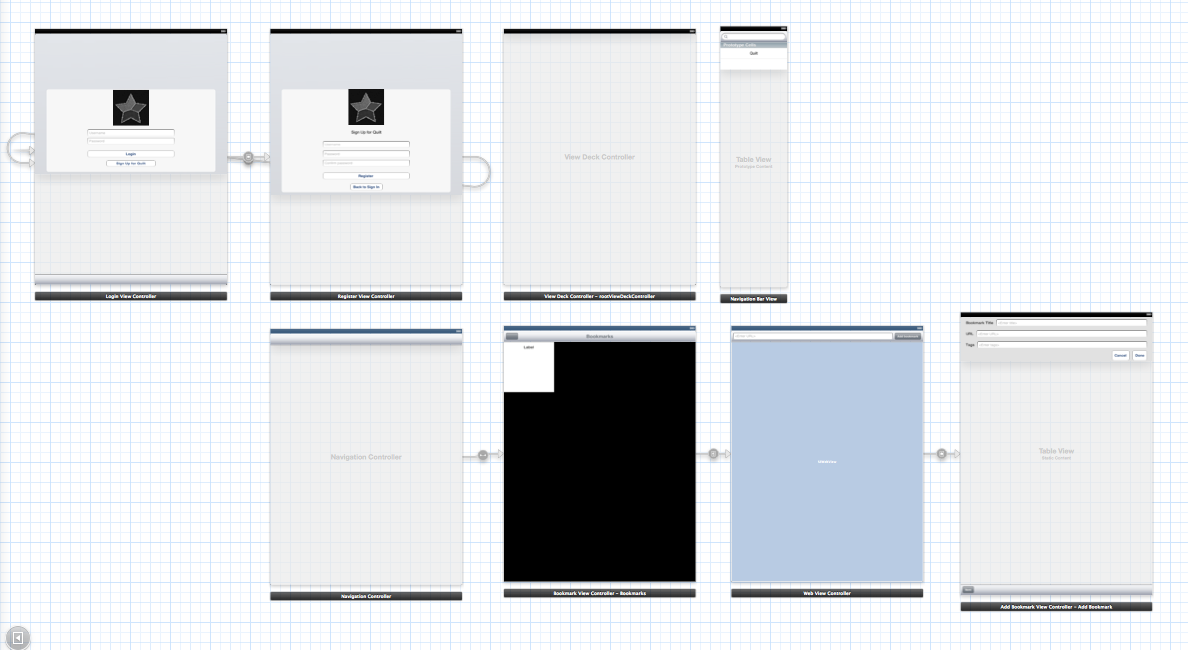
\includegraphics[width=\textwidth]{screenshots/Storyboard}
	\caption{Xcode Storyboard}
\end{figure}

\begin{figure}
        \centering
        \begin{subfigure}[b]{0.4\textwidth}
                \centering
                \includegraphics[width=\textwidth]{"screenshots/In-App Browsing"}
                \caption{Browsing}
        \end{subfigure}%
        ~ %add desired spacing between images, e. g. ~, \quad, \qquad etc.
          %(or a blank line to force the subfigure onto a new line)
        \begin{subfigure}[b]{0.4\textwidth}
                \centering
                \includegraphics[width=\textwidth]{"screenshots/App Browsing"}
                \caption{Adding Bookmarks}
        \end{subfigure}
        \caption{In-Quilt Web Browsing}\label{fig:browse}
\end{figure}

\section{Conclusion}

In conclusion, Quilt is a sleek social application that will enable the users to share websites of interest between their peers with ease. In doing this project we have set up a good relational database and successfully used a variety of tools and features to connect out front-end UI to our back-end code over the network, putting a strong host of design patterns and processes to use. 



iPhone
Safari Extensions Gallery
Alternative browser add ons

	What we have learned

Xcode
pgAdmin

Objective-C
PHP
Networking 
Databases


		Never used Objective-C before.
		More advanced use of databases
	What we would do differently

Design GUI first, we focussed on backend and functionality first. Iteratively improved it. Because learning a new language had to do it this way to understand all the features. So if we were doing it again, we would be able to do this more efficiently. 

Adapting from iPad to iPhone
Adapt art to screen size
Preserve primary functionality


	What we have done
	What we have not done
	What we have learned
		Never used Objective-C before.
		More advanced use of databases
	What we would do differently
	
\section{Acknowledgements}

We would like to extend our thanks to the following people and applications for their assistance in creating this product:

Our primary platform for creating Quilt was XCode. XCode is a proprietary freeware product that allows its users a limited, non-exclusive license to use the Developer Software on Apple-branded computers to develop and test applications and other software. Given this, were we to follow on to produce this product in a commercial setting we would be allowed to with no restriction from this license.

XCode comes with a set of libraries available such as Cocoa and Cocoa Touch used for the user interface. 
%^- Add reference to license below -> up to you if you add more of the license or not

%Ask Richard about the developer license we got off of doc to test the app on the ipad. Need to check if that license would allow us to sell it on the istore or whether we would need to go ahead and get the paid license ourselves to do so. If it is just for project use note this here.


ViewDeck is a sidebar navigation tool created by Tom Adrianssen hosted on GitHub in 2011. We chose ViewDeck because of its clean simplicity, consistency with the 'look and feel' of other Apple apps, and the fact that, as a navigation tool, it accomplished everything we were looking for with the support for the features that we were currently using, such as Storyboarding in XCode. In particular, we chose ViewDeck over alternatives, such as the Facebook style navigation bar by Ben Hall, as it used the latest iOS. If we were to produce Quilt commercially, we would credit Tom Adrianssen within the application documentation [see license below]
%^- this bit is basically fine, just add the reference to the license below


\subsection{Licenses}

\subsubsection{Software License Agreement for XCode}

The licence for XCode falls under proprietary freeware with open source components.

The software licence agreement states:\\
2. Permitted License Uses and Restrictions.
A. Developer Software. Subject to the terms and conditions of this License, you are granted a limited, nonexclusive
license to use the Developer Software on Apple-branded computers to develop and test application
and other software. You may make only as many internal use copies of the Developer Software as
reasonably necessary to use the Developer Software as permitted under this License and distribute such
copies only to your employees whose job duties require them to so use the Developer Software; provided
that you reproduce on each copy of the Developer Software or portion thereof, all copyright or other
proprietary notices contained on the original.

\subsubsection{IIViewDeckController published under the MIT licens:}

Copyright (C) 2011-2013, Tom Adriaenssen\\
Permission is hereby granted, free of charge, to any person obtaining a copy of this software and associated documentation files (the "Software"), to deal in the Software without restriction, including without limitation the rights to use, copy, modify, merge, publish, distribute, sublicense, and/or sell copies of the Software, and to permit persons to whom the Software is furnished to do so, subject to the following conditions:
The above copyright notice and this permission notice shall be included in all copies or substantial portions of the Software.\\
THE SOFTWARE IS PROVIDED "AS IS", WITHOUT WARRANTY OF ANY KIND, EXPRESS OR IMPLIED, INCLUDING BUT NOT LIMITED TO THE WARRANTIES OF MERCHANTABILITY, FITNESS FOR A PARTICULAR PURPOSE AND NONINFRINGEMENT. IN NO EVENT SHALL THE AUTHORS OR COPYRIGHT HOLDERS BE LIABLE FOR ANY CLAIM, DAMAGES OR OTHER LIABILITY, WHETHER IN AN ACTION OF CONTRACT, TORT OR OTHERWISE, ARISING FROM, OUT OF OR IN CONNECTION WITH THE SOFTWARE OR THE USE OR OTHER DEALINGS IN THE SOFTWARE.

\end{document}
